\chapter{Tables and graphs}

\section{Use cases}
\label{sec:use_cases_appendixc}

Below are the different use cases created during the requirements elicitation process.

\subsection{Use case 2 - Topic handling}
\label{subsec:requirements_engineering-use_cases-topic_handling}

This use case describes how an administrator can edit topics. The administrator must be able to delete one or all subscriptions on a topic. Deletion of topics is also included in the use case.

\begin{table}[ht!]
\begin{minipage}{.5\textwidth}
\centering
\resizebox{\textwidth}{!}{
\begin{tabular}{|l|p{5cm}|}
\hline
\textbf{Use case ID} & U2 \\ \hline
\textbf{Use case Name} & Topic handling \\ \hline
\textbf{Description} & Admin should be able to delete topics.  \\ \hline
\textbf{Pre conditions} & The admin is logged in and there exists one or more topics. \\ \hline
\textbf{Standard flow} & \begin{enumerate}
\item Click the topics pane.
\item Click the topic to edit.
\item Alternatives: \begin{enumerate}
    \item Delete one topic.
    \item Delete one subscriber.
    \item Delete all topics.
\end{enumerate}
\end{enumerate} \\ \hline
\textbf{Alternative flow} &  \\ \hline
\textbf{Post conditions} & Subscribers or topics are deleted from the broker.  \\ \hline
\end{tabular}
}
\caption{Use case 2 - Topic handling}
\label{uc2}
\end{minipage}
\hfill
\begin{minipage}{.4\textwidth}
\centering
\begin{center}
    \makebox[\textwidth]{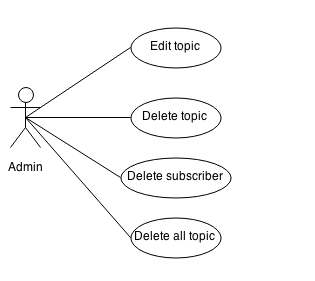
\includegraphics[width=\textwidth]{fig/usecase/usecase_v3_topic.png}}
    \caption{U2 - Topic handling}
    \label{fig:u2}
\end{center}
\end{minipage}
\end{table}

\clearpage

\subsection{Use case 3 - Server information}
\label{subsec:requirements_engineering-use_cases-server_information}

This use case describes how an administrator can view information about the server. This includes server statistics and message brokering statistics. 

\begin{table}[ht!]
\centering
\begin{tabular}{|l|p{5cm}|}
\hline
\textbf{Use case ID} & U3 \\ \hline
\textbf{Use case Name} & Server information. \\ \hline
\textbf{Description} & As an admin I would like to see information and status about the server.  \\ \hline
\textbf{Pre conditions} & The admin is logged in.\\ \hline
\textbf{Standard flow} & \begin{enumerate}
\item Click the pane of interest.
\item Read information on the pane of interest.  
\end{enumerate} \\ \hline
\textbf{Alternative flow} & \\ \hline
\textbf{Post conditions} & The admin has seen the information. \\ \hline
\end{tabular}
\caption{Use case 3 - Server information}
\label{uc3}
\end{table}

\begin{center}
  \begin{figure}[ht!]
    \makebox[\textwidth]{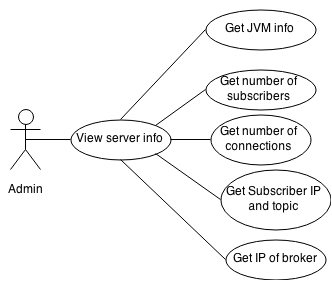
\includegraphics[width=6cm]{fig/usecase/usecase_v3_serverinfo.png}}
    \caption{U3 - Server information}
    \label{fig:u3}
  \end{figure}
\end{center}

\clearpage

\subsection{Use case 4 - Log in}
\label{subsec:requirements_engineering-use_cases-log_in}

The following describes the log in procedure. The group concluded that no other functions were needed than a simple username and password log in function. Recover password were not included due to there being little to no persistent data in the database. Thus, a new instance could be initiated instead.

\begin{table}[ht!]
\centering
\begin{tabular}{|l|p{5cm}|}
\hline
\textbf{Use case ID} & U2 \\ \hline
\textbf{Use case Name} & Log in \\ \hline
\textbf{Description} & As an Admin I would like to log in to the admin console. \\ \hline
\textbf{Pre conditions} & The admin is not logged in. \\ \hline
\textbf{Standard flow} & \begin{enumerate}
\item Inserts username and password.
\item Clicks "Log in".
\item Enter the admin console. 
\end{enumerate} \\ \hline
\textbf{Alternative flow} & \begin{description}
\item[2A:] The username or password is wrong. \begin{enumerate}
\item Redirect user to front page.
\item Display error message.
\end{enumerate}
\end{description} \\ \hline
\textbf{Post conditions} & Admin logged in. \\ \hline
\end{tabular}
\caption{Use case 4 - Log in}
\label{uc4}
\end{table}

\begin{center}
  \begin{figure}[ht!]
    \makebox[\textwidth]{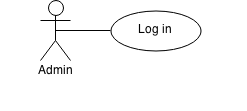
\includegraphics[width=6cm]{fig/usecase/usecase1.png}}
    \caption{U4 - Log in}
    \label{fig:u4}
  \end{figure}
\end{center}

\subsection{Use case 5 - Message sending}
\label{subsec:requirements_engineering-use_cases-message_sending}

This use case attempts to capture the process of sending messages over the system. This only captures a simplified version of the message sending. Some variations occur from protocol to protocol.

\begin{table}[ht!]
\centering
\begin{tabular}{|l|p{5cm}|}
\hline
\textbf{Use case ID} & U5 \\ \hline
\textbf{Use case Name} & Message sending \\ \hline
\textbf{Description} & User should be able to send a message over a protocol.  \\ \hline
\textbf{Pre conditions} &  \\ \hline
\textbf{Standard flow} & \begin{enumerate}
\item Register as a publisher on a topic.
\item Send the message.
\end{enumerate} \\ \hline
\textbf{Alternative flow} & \begin{enumerate}
\item [1A:] Topic is protected.
\item User registers as publisher with username and password.
\end{enumerate} \\ \hline
\textbf{Post conditions} & Message is sent.  \\ \hline
\end{tabular}
\caption{Use case 5 - Message sending}
\label{uc5}
\end{table}

\begin{center}
  \begin{figure}[ht!]
    \makebox[\textwidth]{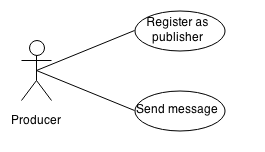
\includegraphics[width=6cm]{fig/usecase/fig44.png}}
    \caption{U5 - Message sending}
    \label{fig:u5}
  \end{figure}
\end{center}

\clearpage

\subsection{Use case 6 - Message Receiving}
\label{subsec:requirements_engineering-use_cases-message_recieving}

This use case attempts to capture the process of receiving messages over the system. This only captures a simplified version of the message retrieval. Some variations occur from protocol to protocol.

\begin{table}[ht!]
\centering
\begin{tabular}{|l|p{5cm}|}
\hline
\textbf{Use case ID} & U6 \\ \hline
\textbf{Use case Name} & Receiving messages. \\ \hline
\textbf{Description} & User should be able to receive a message over a protocol.  \\ \hline
\textbf{Pre conditions} & The message is sent. \\ \hline
\textbf{Standard flow} & \begin{enumerate}
\item Register as a subscriber on a topic.
\item Receive the message.
\end{enumerate} \\ \hline
\textbf{Alternative flow} & \\ \hline
\textbf{Post conditions} & Message has been received.  \\ \hline
\end{tabular}
\caption{Use case 6 - Message retrieval}
\label{uc6}
\end{table}

\begin{center}
  \begin{figure}[ht!]
    \makebox[\textwidth]{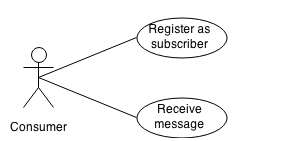
\includegraphics[width=6cm]{fig/usecase/fig45.png}}
    \caption{U6 - Message retrieval}
    \label{fig:u6}
  \end{figure}
\end{center}
\clearpage

\subsection{Use case 7 - Subscribe with WSN}
\label{subsec:requirements_engineering-use_cases-sub_wsn}

This use case attempts to capture the process of subscribing to a topic using the WSN protocol. 

\begin{table}[ht!]
\centering
\begin{tabular}{|l|p{5cm}|}
\hline
\textbf{Use case ID} & U7 \\ \hline
\textbf{Use case Name} & Subscribe with WSN. \\ \hline
\textbf{Description} & A consumer should be able to subscribe to a topic using the WSN protocol.  \\ \hline
\textbf{Pre conditions} & OKSE broker is up and running. \\ \hline
\textbf{Standard flow} & \begin{enumerate}
\item Send subscription request to OKSE.
\end{enumerate} \\ \hline
\textbf{Alternative flow} & \\ \hline
\textbf{Post conditions} & The consumer is now subscribed to the requested topic.  \\ \hline
\end{tabular}
\caption{Use case 7 - Subscribe with WSN}
\label{uc7}
\end{table}

\begin{center}
  \begin{figure}[ht!]
    \makebox[\textwidth]{\includegraphics[width=6cm]{}}
    \caption{U7 - Subscribe with WSN}
    \label{fig:u7}
  \end{figure}
\end{center}
\clearpage

\subsection{Use case 8 - Register as a publisher on a topic with WSN}
\label{subsec:requirements_engineering-use_cases-reg_pub_wsn}

Use case showing how to register as a publisher on a topic using the WSN protocol 

\begin{table}[ht!]
\centering
\begin{tabular}{|l|p{5cm}|}
\hline
\textbf{Use case ID} & U8 \\ \hline
\textbf{Use case Name} & Register producer WSN. \\ \hline
\textbf{Description} & A client should be able to register as publisher on a topic with the WSN protocol.  \\ \hline
\textbf{Pre conditions} & OKSE broker is up and running. \\ \hline
\textbf{Standard flow} & \begin{enumerate}
\item Send request to OKSE.
\item Receive registration confirmation.
\end{enumerate} \\ \hline
\textbf{Alternative flow} & \\ \hline
\textbf{Post conditions} & Client is now registered as a publisher on the requested topic. 
  \\ \hline
\end{tabular}
\caption{Use case 8 - Register producer WSN}
\label{uc8}
\end{table}

\begin{center}
  \begin{figure}[ht!]
    \makebox[\textwidth]{\includegraphics[width=6cm]{}}
    \caption{U8 - Register producer WSN}
    \label{fig:u8}
  \end{figure}
\end{center}

\clearpage

\subsection{Use case 9 - Unsubscribe with WSN}
\label{subsec:requirements_engineering-use_cases-unsub_wsn}

Use case showing how to unsubscribe from a topic using the WSN protocol. 

\begin{table}[ht!]
\centering
\begin{tabular}{|l|p{5cm}|}
\hline
\textbf{Use case ID} & U9 \\ \hline
\textbf{Use case Name} & Unsubscribe with WSN. \\ \hline
\textbf{Description} & A user must be able to unsubscribe for a topic using the WSN protocol.  \\ \hline
\textbf{Pre conditions} & OKSE broker is up and running. The user has an active subscription on the topic which the user wants to 	unsubscribe from. \\ \hline
\textbf{Standard flow} & \begin{enumerate}
\item Send unsubscribe request to OKSE.
\item Receive unsubscribe confirmation.
\end{enumerate} \\ \hline
\textbf{Alternative flow} & \\ \hline
\textbf{Post conditions} & The user is now unsubscribed from requested topic and will no longer receive messages sent on that topic. 
  \\ \hline
\end{tabular}
\caption{Use case 9 - Unsubscribe from topic WSN}
\label{uc9}
\end{table}

\begin{center}
  \begin{figure}[ht!]
    \makebox[\textwidth]{\includegraphics[width=6cm]{}}
    \caption{U9 - Unsubscribe from topic WSN}
    \label{fig:u9}
  \end{figure}
\end{center}

\clearpage

\subsection{Use case 10 - Unregister as a publisher on a topic wih WSN.}
\label{subsec:requirements_engineering-use_cases-unreg_pub}

Use case showing how to unregister as a publisher using the WSN protocol. 

\begin{table}[ht!]
\centering
\begin{tabular}{|l|p{5cm}|}
\hline
\textbf{Use case ID} & U10 \\ \hline
\textbf{Use case Name} & Unregister as publisher with WSN. \\ \hline
\textbf{Description} & A user must be able to unregister as a publisher on a topic using the WSN protocol.  \\ \hline
\textbf{Pre conditions} & OKSE broker is up and running. The user is registered as a publisher on the topic which the user wants to unsubscribe from.  \\ \hline
\textbf{Standard flow} & \begin{enumerate}
\item Send unregister request to OKSE.
\item Receive unregister confirmation.
\end{enumerate} \\ \hline
\textbf{Alternative flow} & \\ \hline
\textbf{Post conditions} & The user is now unregistered as a publisher on the requested topic. 
  \\ \hline
\end{tabular}
\caption{Use case 10 - Unregister as publisher using WSN}
\label{uc10}
\end{table}

\begin{center}
  \begin{figure}[ht!]
    \makebox[\textwidth]{\includegraphics[width=6cm]{}}
    \caption{U10 - Unregister as publisher using WSN}
    \label{fig:u10}
  \end{figure}
\end{center}

\clearpage

\subsection{Use case 11 - Retrieve the latest message on a topic using the GetCurrentMessage function with WSN.}
\label{subsec:requirements_engineering-use_cases-get_message_wsn}

Use case showing how to retrieve the latest message on a topic using the GetCurrentMessage function.


\begin{table}[ht!]
\centering
\begin{tabular}{|l|p{5cm}|}
\hline
\textbf{Use case ID} & U11 \\ \hline
\textbf{Use case Name} & Get latest message on topic using WSN.\\ \hline
\textbf{Description} & A user must be able to get the last message sent on a topic using the WSN protocol\\ \hline
\textbf{Pre conditions} & OKSE broker is up and running. There is a message to retrieve.\\ \hline
\textbf{Standard flow} & \begin{enumerate}
\item Send request using GetCurrentMessage to OKSE using WSN.
\item Receive last message sent on requested topic.
\end{enumerate} \\ \hline
\textbf{Alternative flow} & \\ \hline
\textbf{Post conditions} & User now has local copy of last message sent on requested topic  
  \\ \hline
\end{tabular}
\caption{Use case 11 - GetCurrentMessage function with WSN}
\label{uc11}
\end{table}

\begin{center}
  \begin{figure}[ht!]
    \makebox[\textwidth]{\includegraphics[width=6cm]{}}
    \caption{U11 - GetCurrentMessage function with WSN}
    \label{fig:u11}
  \end{figure}
\end{center}

\clearpage

\subsection{Use case 12 - Renew subscription using the WSN protocol}
\label{subsec:requirements_engineering-use_cases-renew_sub_wsn}

Use case showing the steps involved in renewing subscription on topic with WSN. 

\begin{table}[ht!]
\centering
\begin{tabular}{|l|p{5cm}|}
\hline
\textbf{Use case ID} & U12 \\ \hline
\textbf{Use case Name} & Renew subscription using WSN protocol.\\ \hline
\textbf{Description} & A user should be able to renew subscription on a requested topic using WSN protocol.\\ \hline
\textbf{Pre conditions} & OKSE is up and running. The user has an active subscription on the topic which he/she wants to renew.\\ \hline
\textbf{Standard flow} & \begin{enumerate}
\item Send request to OKSE with new timeout date. 
\item Receive confirmation from OKSE with updated subscription timeout date.
\end{enumerate} \\ \hline
\textbf{Alternative flow} & \\ \hline
\textbf{Post conditions} & The user will have a updated timeout date for the subscription on the requested topic.\\ \hline
\end{tabular}
\caption{Use case 12 - Renew subscription using WSN}
\label{uc12}
\end{table}

\begin{center}
  \begin{figure}[ht!]
    \makebox[\textwidth]{\includegraphics[width=6cm]{}}
    \caption{U12 - Renew subscription using WSN}
    \label{fig:u12}
  \end{figure}
\end{center}

\clearpage

\subsection{Use case 13 - Pause subscription using the WSN protocol}
\label{subsec:requirements_engineering-use_cases-pause_sub_wsn}

Use case showing the steps involved in pausing subscription on topic with WSN. 

\begin{table}[ht!]
\centering
\begin{tabular}{|l|p{5cm}|}
\hline
\textbf{Use case ID} & U13 \\ \hline
\textbf{Use case Name} & Pause subscription using WSN protocol.\\ \hline
\textbf{Description} & The user should be able to pause a subscription on a requested topic using the WSN protocol. \\ \hline
\textbf{Pre conditions} & OKSE is up and running. User must have active subscription on the topic which he/she wants to pause\\ \hline
\textbf{Standard flow} & \begin{enumerate}
\item Send request to OKSE. 
\item Receive confirmation from OKSE.
\end{enumerate} \\ \hline
\textbf{Alternative flow} & \\ \hline
\textbf{Post conditions} & Subscription is now on pause. User will no longer receive messages sent on that topic. Subscription is not removed from OKSE\\ \hline
\end{tabular}
\caption{Use case 13 - Pause subscription using WSN}
\label{uc13}
\end{table}

\begin{center}
  \begin{figure}[ht!]
    \makebox[\textwidth]{\includegraphics[width=6cm]{}}
    \caption{U13 - Pause subscription using WSN}
    \label{fig:u13}
  \end{figure}
\end{center}

\clearpage

\subsection{Use case 14 - Resume subscription using the WSN}
\label{subsec:requirements_engineering-use_cases-resume_sub_wsn}

Use case showing the steps involved in resuming a paused subscription on topic with WSN. 

\begin{table}[ht!]
\centering
\begin{tabular}{|l|p{5cm}|}
\hline
\textbf{Use case ID} & U14 \\ \hline
\textbf{Use case Name} & Resume subscription with WSN protocol\\ \hline
\textbf{Description} & The user should be able to resume a subscription on a topic which previously was paused. \\ \hline
\textbf{Pre conditions} & OKSE is up and running. User has a paused subscription on the topic which he/she wants to resume. \\ \hline
\textbf{Standard flow} & \begin{enumerate}
\item Send request to OKSE
\item Receive confirmation from OKSE	
\end{enumerate} \\ \hline
\textbf{Alternative flow} & \\ \hline
\textbf{Post conditions} & The subscription on the requested topic is resumed. The user will now receive messages sent on the topic which the user resumed subscription on.  \\ \hline
\end{tabular}
\caption{Use case 14 - Resume subscription with WSN}
\label{uc14}
\end{table}

\begin{center}
  \begin{figure}[ht!]
    \makebox[\textwidth]{\includegraphics[width=6cm]{}}
    \caption{U14 - Resume subscription with WSN}
    \label{fig:u14}
  \end{figure}
\end{center}

\clearpage

\subsection{Use case 15 - }
\label{subsec:requirements_engineering-use_cases-}

Use case showing the steps involved 

\begin{table}[ht!]
\centering
\begin{tabular}{|l|p{5cm}|}
\hline
\textbf{Use case ID} & U15 \\ \hline
\textbf{Use case Name} & \\ \hline
\textbf{Description} & \\ \hline
\textbf{Pre conditions} & \\ \hline
\textbf{Standard flow} & \begin{enumerate}
\item 
\item 	
\end{enumerate} \\ \hline
\textbf{Alternative flow} & \\ \hline
\textbf{Post conditions} & \\ \hline
\end{tabular}
\caption{Use case 15 - }
\label{uc15}
\end{table}

\begin{center}
  \begin{figure}[ht!]
    \makebox[\textwidth]{\includegraphics[width=6cm]{}}
    \caption{U15 - }
    \label{fig:u15}
  \end{figure}
\end{center}

\clearpage

\section{Testing}

\subsection{Integration testing test cases}

\begin{table}[ht!]
\tiny
\begin{tabular}{|m{0.5cm}|m{1.5cm}|m{1.5cm}|m{3cm}|m{3cm}|m{1.5cm}|}
\hline
\rowcolor{lightgray}
\textbf{ID} & \textbf{Service/Protocol} & \textbf{Method} & \textbf{Procedure} & \textbf{Expected} & \textbf{Result}\\ \hline
IT1.1 & CoreService & boot & Start the Application & Thread running and all registered services alive & Success \\ \hline
IT1.2 & CoreService & stop & Stop the Application & All registered services shut down and threads killed. Invoked flags set to false. CoreService thread removed and invoked flag set to false. & Success \\ \hline
IT1.3 &CoreService & execute & Create and insert a runnable job to the executor service using the execute method & Job successfully performed & Success \\ \hline
IT1.4 & CoreService & registerService & Initialize a stub abstractcoreservice and register it to the CoreService & Stub service is correctly registered & Success \\ \hline
IT1.5 & CoreService & removeService & Perform IT1.4 and then remove the service again & Service correctly removed & Success \\ \hline
IT1.6 & CoreService & addProtocolServer & Register the DummyProtocolServer & DummyProtocolServer correctly added to list of protocol servers & Success \\ \hline
IT1.7 & CoreService & removeProtocolServer & Perform IT1.6 and then remove the protocol server again & Protocol server correctly removed & Success \\ \hline
IT1.8 & CoreService & getTotalRequests FromProtocolServers & Perform a request using DummuProtocolServer and verify counter increment in admin panel & Request counter incremented by 1 per request & Success \\ \hline
IT1.9 & CoreService & getTotalMessages RecievedFromProtocolServers & Increment the DummyProtocol's recieved messages field & Messages recieved counter incremented by 1 per message & Success \\ \hline
IT1.10 & CoreService & getTotalMessages SentFromProtocolServers & Increment the DummyProtocol's sent messages field & Messages sent counter incremented by 1 per message & Success \\ \hline
IT1.11 & CoreService & getTotalBadRequests FromProtocolServers & Write jibberish using the DummyProtocol telnet command interface & Bad requests counter incremented by 1 per bad request sent & Success \\ \hline
IT1.12 & CoreService & getTotalErrors FromProtocolServers & Increment the DummyProtocol's total errors field & Total errors counter incremented by 1 per error & Success \\ \hline
IT1.13 & CoreService & getAllProtocolServers & Perform IT6.1 and verify that it is returned from the method & Set of registered protocol servers increased by 1 during registry, and DummyProtocolServer included in the shallow copy hash set returned. & Success \\ \hline
IT1.14 & CoreService & getProtocolServer & Perform IT6.1 and then provide the Class type of the DummyProtocolServer as an argument. & The instance of DummyProtocolServer successfully returned & Success \\ \hline
IT1.15 & CoreService & stopAllProtocol Servers & Call the method from test class & All protocol servers gracefully shut down, their threads removed and invoked flag set to false. & ? \\ \hline
IT1.16 & CoreService & bootCoreServices & Perform 1.4 twice using 2 different stubs. Then call the method. & Both registered stub services booted successfully in their own thread, with run and invoked flags set to true. & Success \\ \hline
IT1.17 & CoreService & bootProtocolServers & Perform IT1.6 then call the method & DummyProtocoLServer successfully booted in its own thread, with run and invoked flags set to true. & Success \\ \hline
IT1.18 & CoreService & registerListenerSupport ForAllCoreServices & Perform IT1.4 with debug output in its registerListenerSupport method. Then invoke the test method & Debug output successfully displayed when method is invoked. & Success \\ \hline
\end{tabular}
\caption{Integration Testing - Test Cases}
\label{table:integration-testing-cases}
\end{table}

\section{System testing test cases}

\clearpage

\end{appendices}